\section{Organizational Breakdown Structure}
\label{dsePPOBS}
The organizational breakdown can be found in figure \ref{organogram} on page \pageref{organogram}. The diagram has been divided into two logical parts: management and technical responsibilities.

The managerial responsibilities are as follows:
\begin{itemize}
	\item Chairman - responsible for keeping the project on track and is accountable for all deliverables. He is furthermore entrusted with making sure all the meetings are organized and that all members are aware of what they are supposed to be doing.
	\item Secretary - keeps track of all discussions and decisions made at meetings. Furthermore he is responsible for communications with the tutor as well as logistics.
	\item System Engineer - person responsible for correctness of system engineering content.
	\item Archiver - responsible for organizing and overseeing IT resources to be used for data storage and report writing.
	\item Quality Assurer - responsible for report content.
	\item External Relations - responsible for contact with external parties.
	\item Sustainable Engineer - responsible for sustainable development guidance. 
\end{itemize}

%\newpage
\begin{figure}[H]
\begin{center}

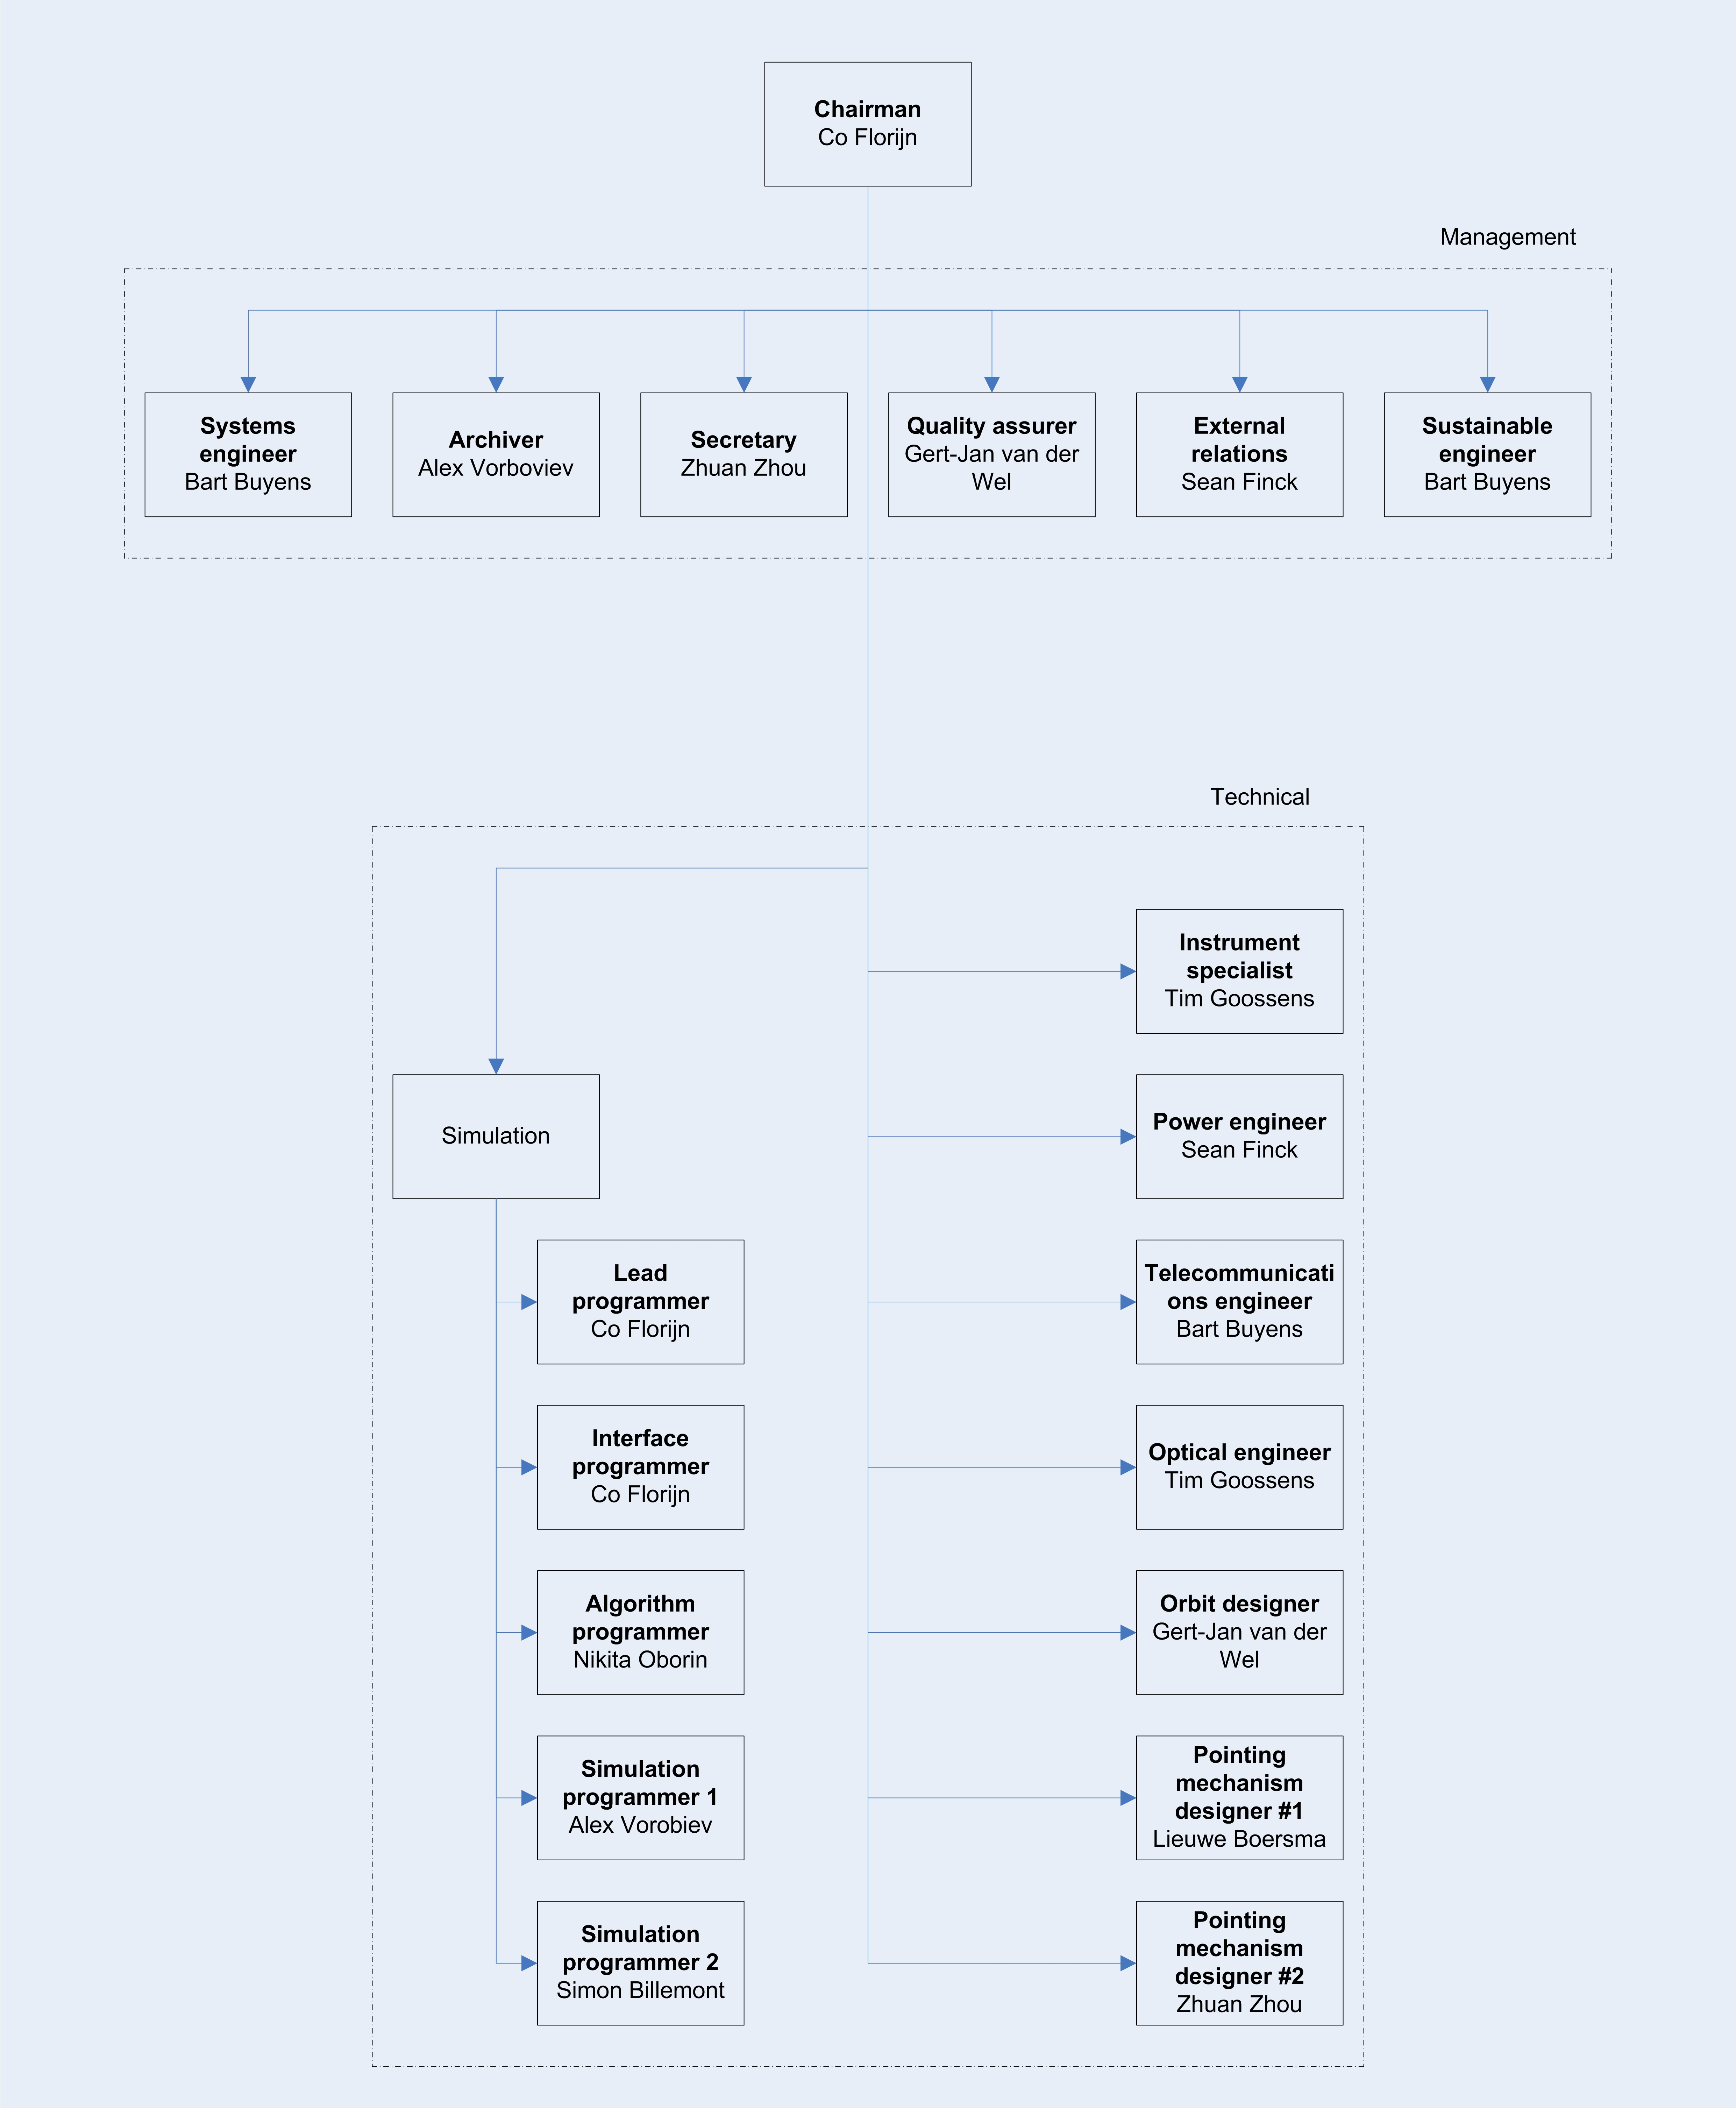
\includegraphics[scale=0.8]{chapters/img/Organogram.jpg}
\caption{Organogram}
\label{organogram}
\end{center}
\end{figure}